\section{Simulation Results}

%%% 6-by-6 3 agents r3 no obs
\begin{figure}[H]
  \centering
  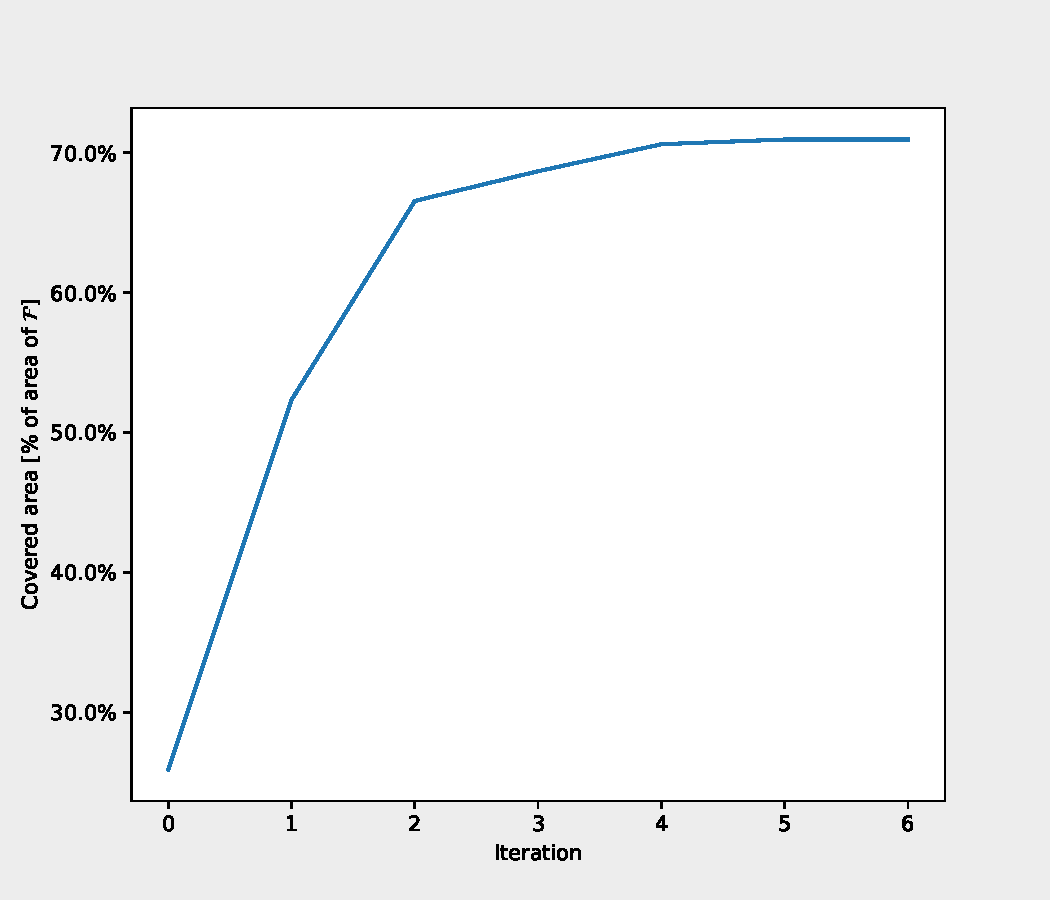
\includegraphics[width=.75\textwidth]{figs/6_by_6_no_obs_3_agnts_area_traj.pdf}
  \caption{Percentage covered area of $\mathcal{F}$ vs. iteration count for rectangular environment. Area of $\mathcal{F} = 36\:\mathrm{m}^{2}$}
  \label[fig]{local_coverage_example}
\end{figure}
\begin{figure}[H]
  \centering
  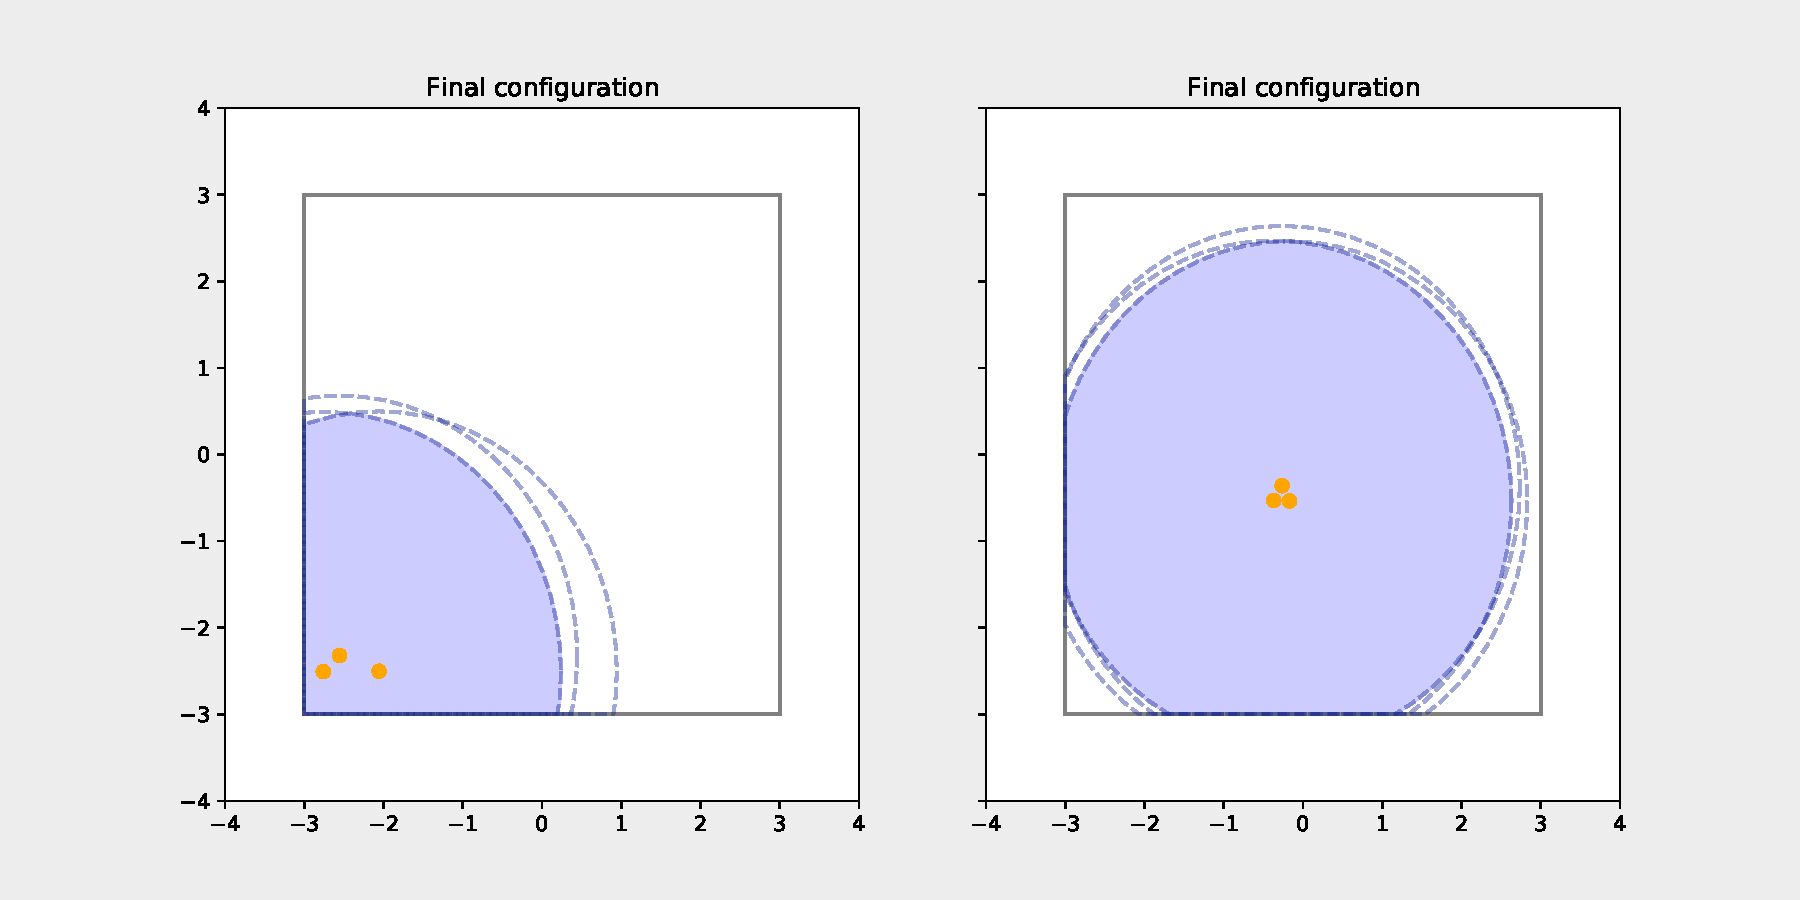
\includegraphics[width=.75\textwidth]{figs/6_by_6_no_obs_3_agnts_distr.pdf}
  \caption{Inital and final position of agents in rectangular environment. Area of $\mathcal{F} = 36\:\mathrm{m}^{2}$, maximum communication range $r=3\:\mathrm{m}$.}
  \label[fig]{local_coverage_example}
\end{figure}

%%% 6-by-6 10 agents r3 no obs
\begin{figure}[H]
  \centering
  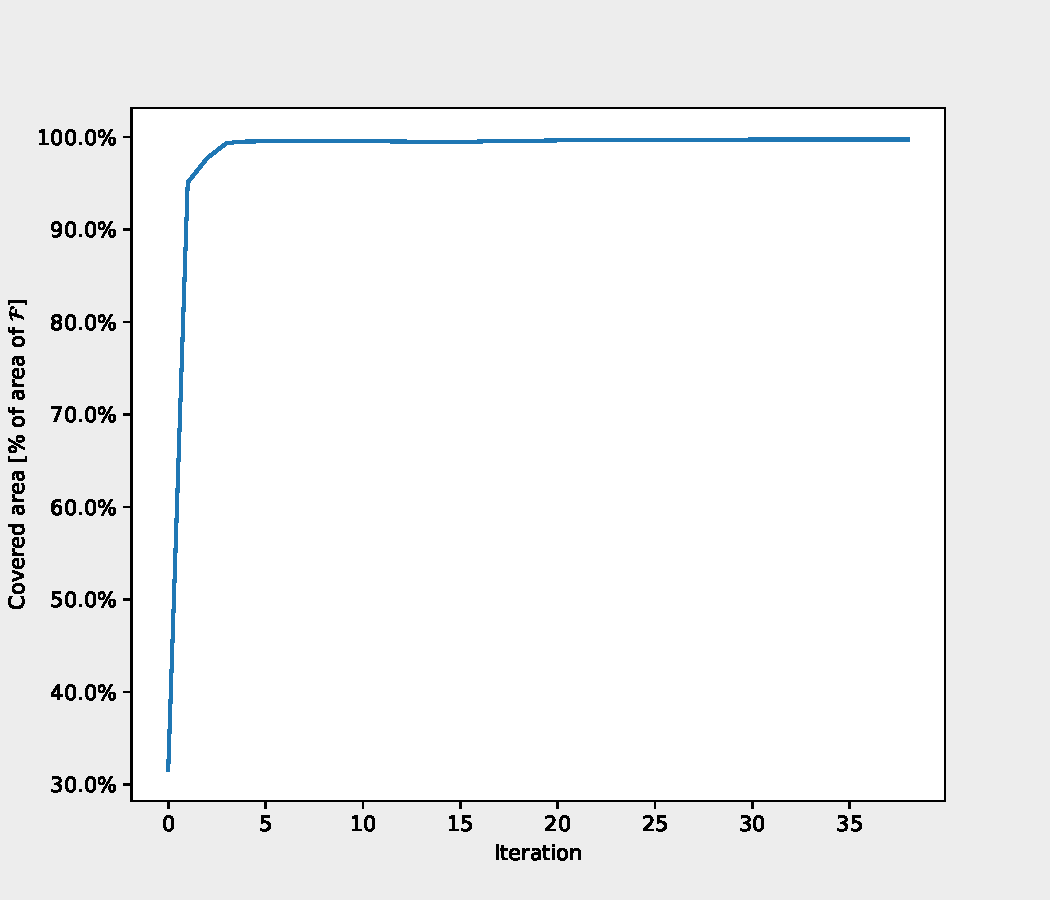
\includegraphics[width=.75\textwidth]{figs/6_by_6_no_obs_10_agnts_area_traj.pdf}
  \caption{Percentage covered area of $\mathcal{F}$ vs. iteration count for rectangular environment with rectangular central obstacle. Area of $\mathcal{F} = 36\:\mathrm{m}^{2}$}
  \label[fig]{local_coverage_example}
\end{figure}
\begin{figure}[H]
  \centering
  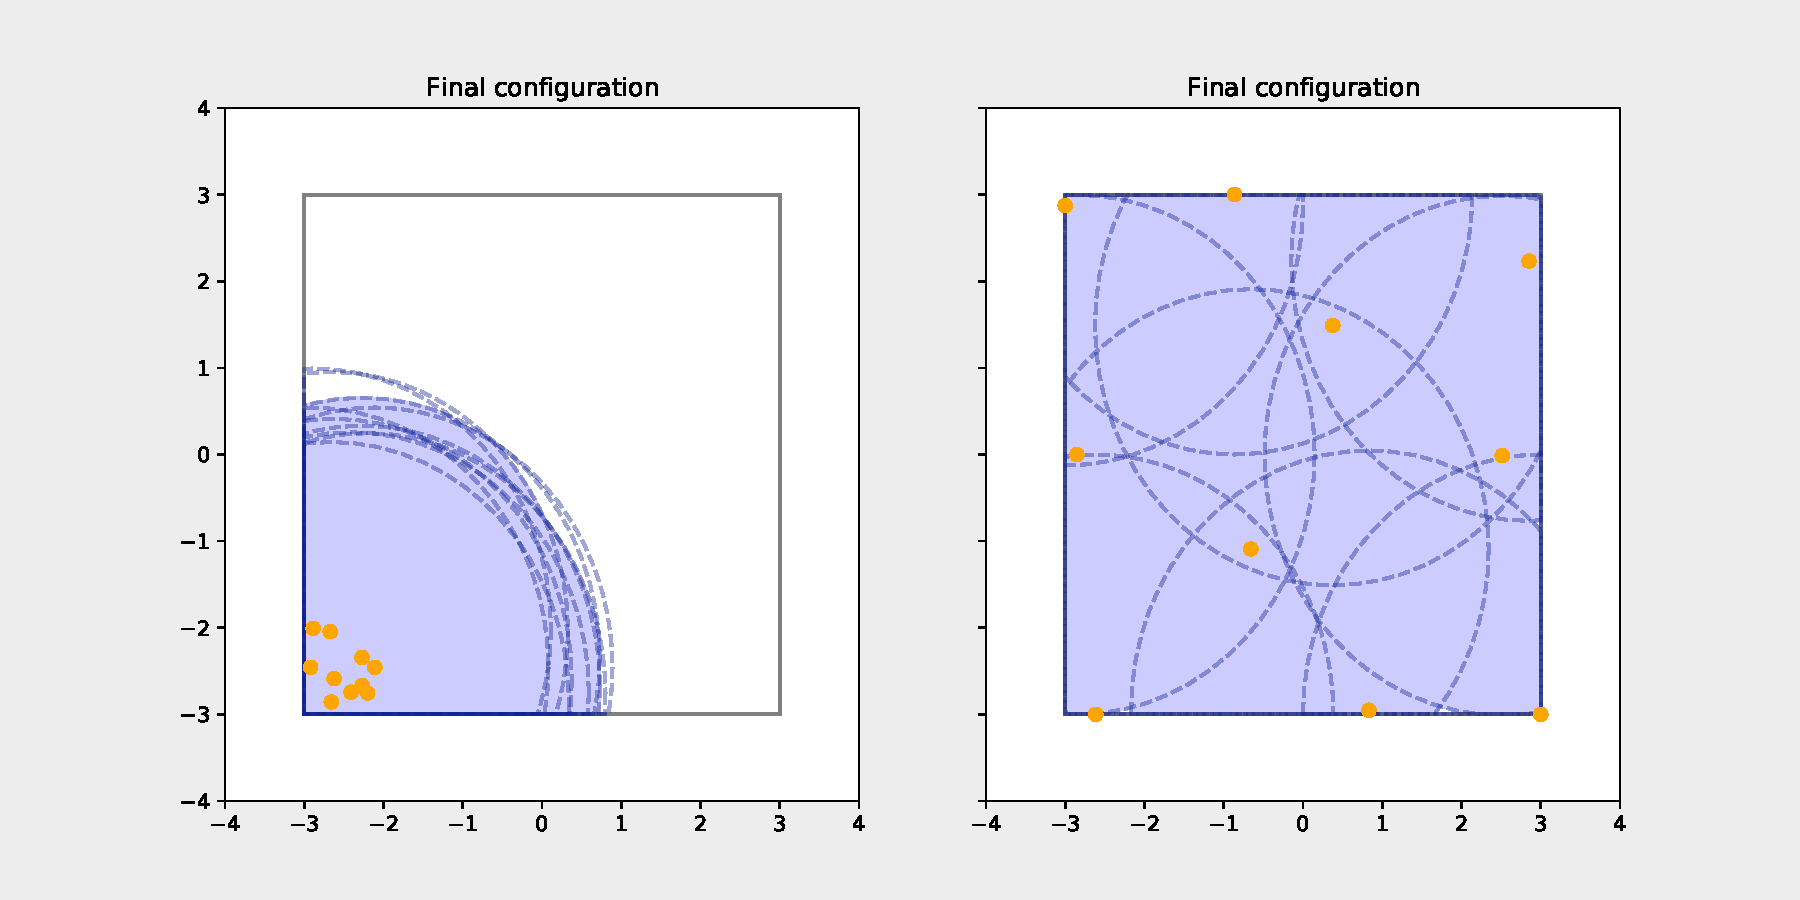
\includegraphics[width=.75\textwidth]{figs/6_by_6_no_obs_10_agnts_distr.pdf}
  \caption{Inital and final position of agents in rectangular environment with rectangular central obstacle. Area of $\mathcal{F} = 36\:\mathrm{m}^{2}$, maximum communication range $r=3\:\mathrm{m}$.}
  \label[fig]{local_coverage_example}
\end{figure}


%%% 2-by-2 Three agents r3
\begin{figure}[H]
  \centering
  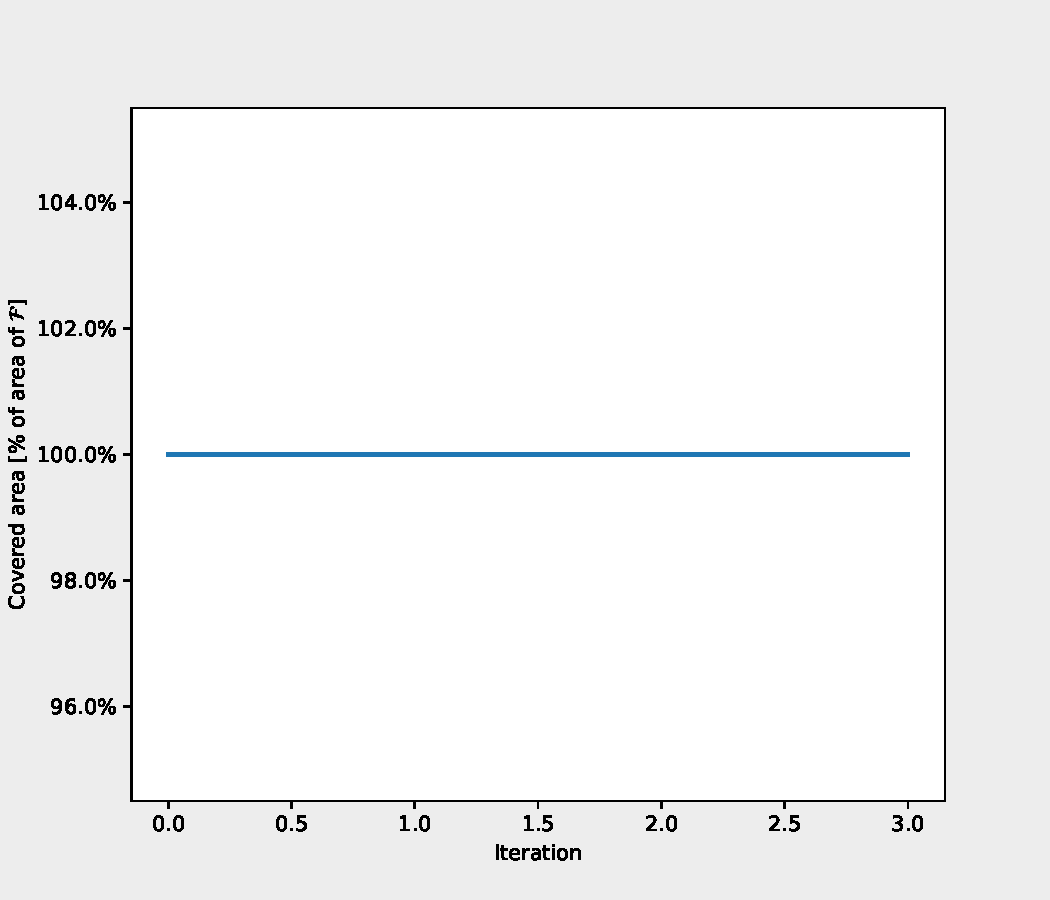
\includegraphics[width=.75\textwidth]{figs/1_by_1_no_obs_3_agnts_area_traj.pdf}
  \caption{Percentage covered area of $\mathcal{F}$ vs. iteration count for rectangular obstacle-less environment. Area of $\mathcal{F} = 4\:\mathrm{m}^{2}$}
  \label[fig]{local_coverage_example}
\end{figure}
\begin{figure}[H]
  \centering
  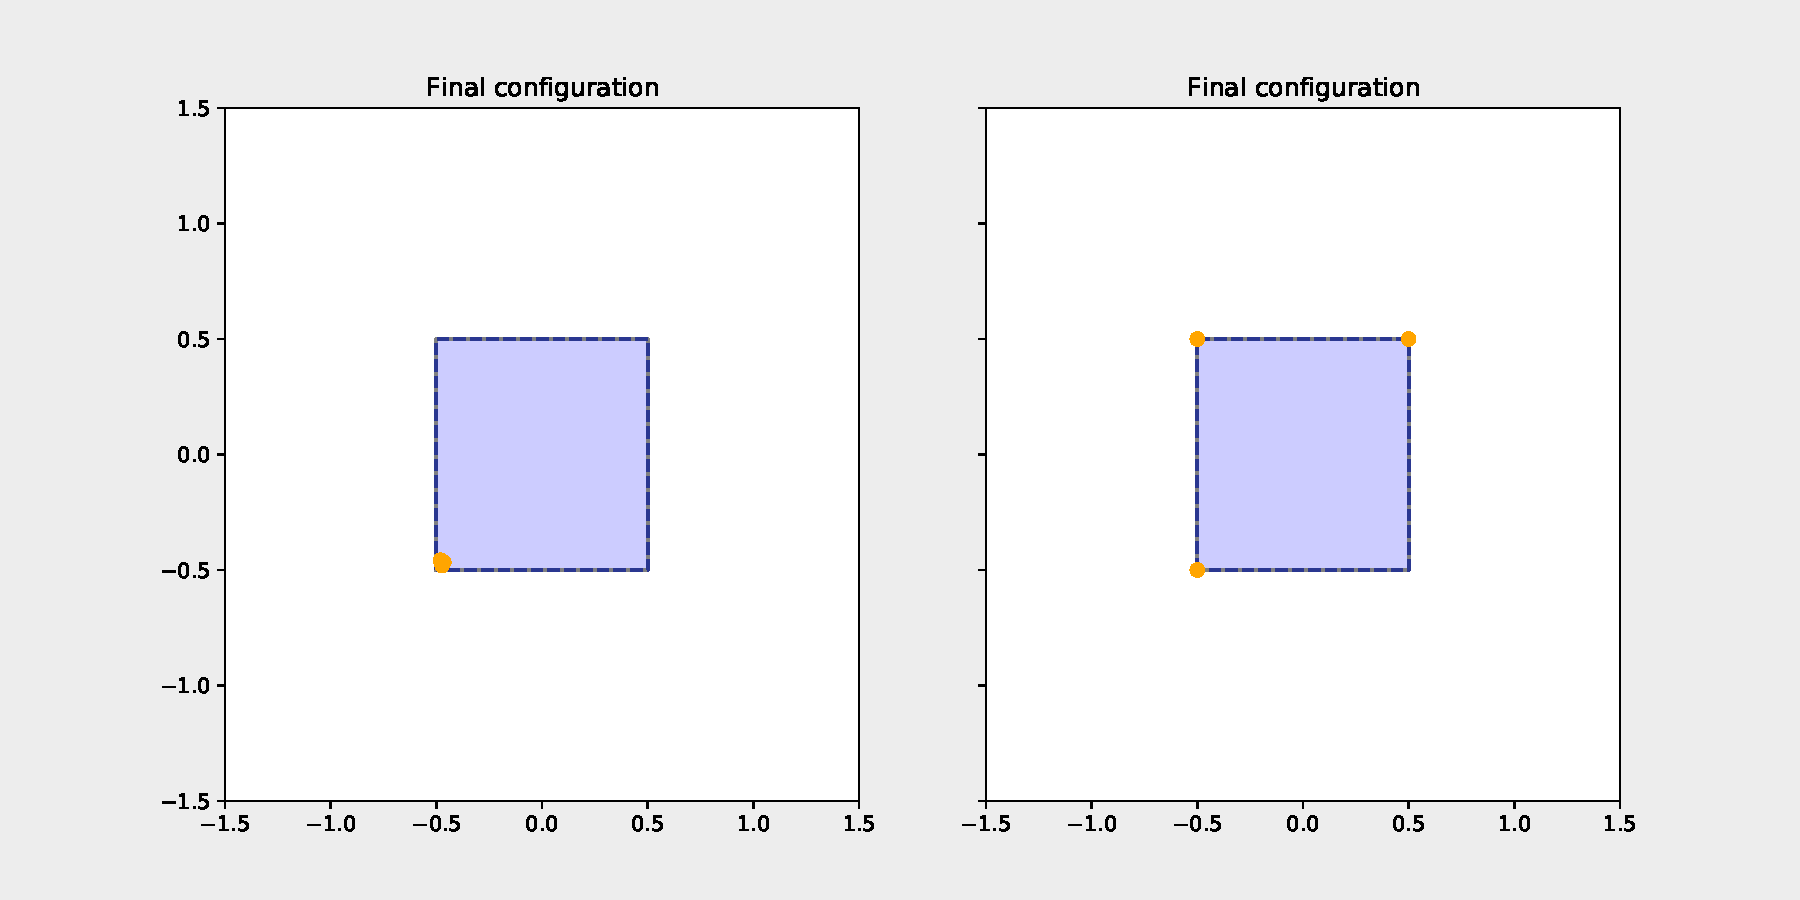
\includegraphics[width=.75\textwidth]{figs/1_by_1_no_obs_3_agnts_distr.pdf}
  \caption{Inital and final position of agents in rectangular obstacle-less environment. Area of $\mathcal{F} = 4\:\mathrm{m}^{2}$, maximum communication range $r=9\:\mathrm{m}$.}
  \label[fig]{local_coverage_example}
\end{figure}

%%% 2-by-2 Three agents r3 center obs
\begin{figure}[H]
  \centering
  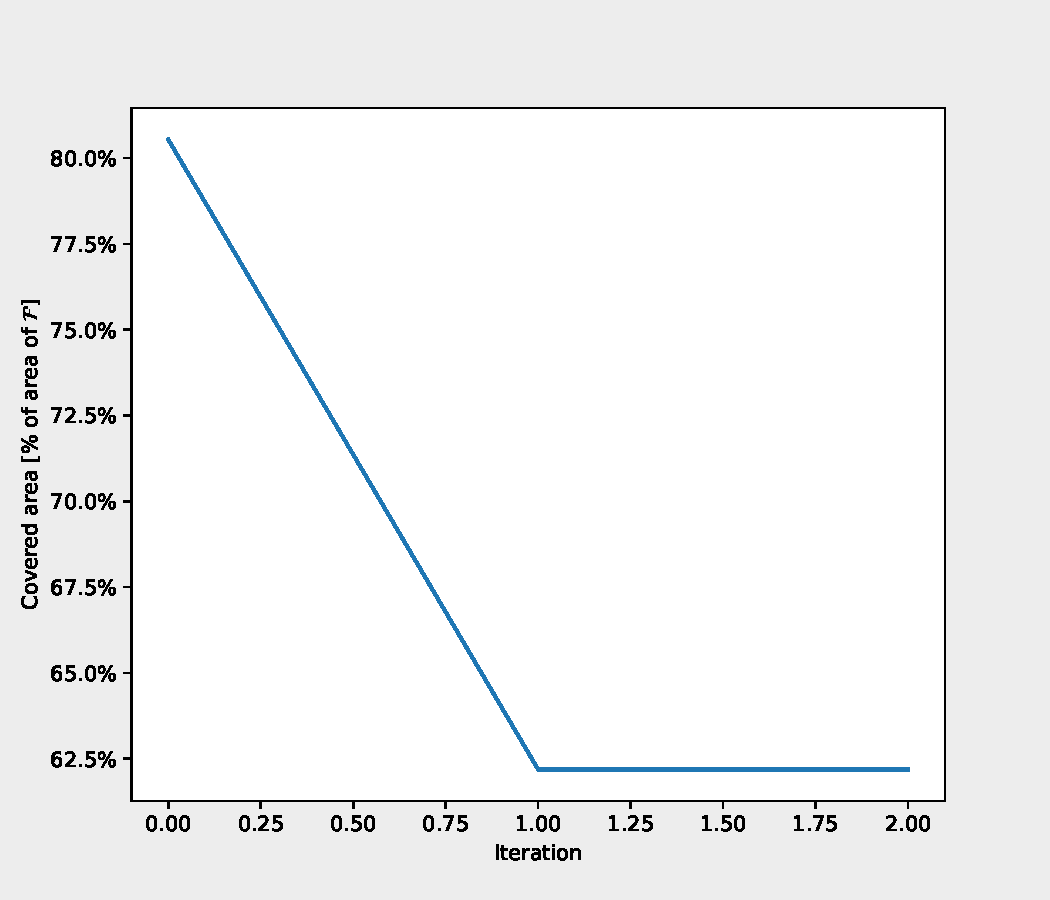
\includegraphics[width=.75\textwidth]{figs/1_by_1_center_obs_3_agnts_area_traj.pdf}
  \caption{Percentage covered area of $\mathcal{F}$ vs. iteration count for rectangular environment with rectangular central obstacle. Area of $\mathcal{F} = 4\:\mathrm{m}^{2}$}
  \label[fig]{local_coverage_example}
\end{figure}
\begin{figure}[H]
  \centering
  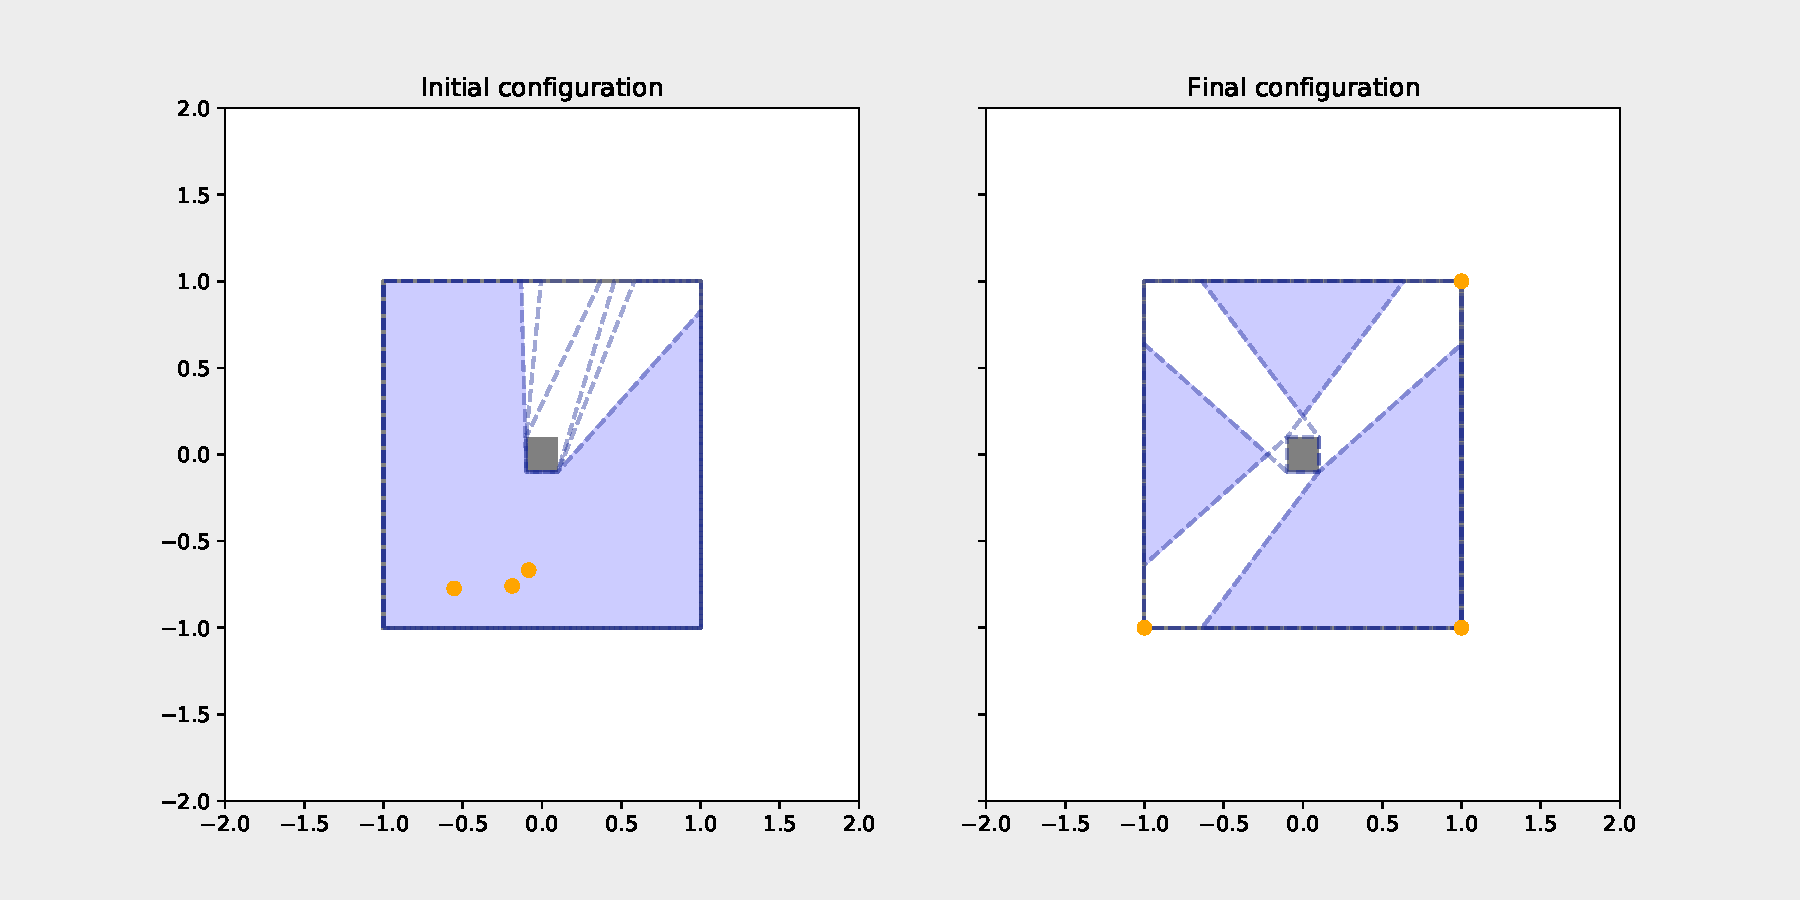
\includegraphics[width=.75\textwidth]{figs/1_by_1_center_obs_3_agnts_distr.pdf}
  \caption{Inital and final position of agents in rectangular environment with rectangular central obstacle. Area of $\mathcal{F} = 4\:\mathrm{m}^{2}$, maximum communication range $r=9\:\mathrm{m}$.}
  \label[fig]{local_coverage_example}
\end{figure}